\documentclass[a4paper,12pt]{article}

\usepackage[utf8]{inputenc}
\usepackage{graphicx}
\usepackage[dvipsnames]{xcolor}

%\usepackage[defaultmono]{droidmono}
\usepackage{wrapfig}
\usepackage{caption}
\usepackage{subcaption}

\usepackage{amsmath,amssymb,amsthm,textcomp}
\usepackage{ dsfont }
\usepackage{enumerate}
\usepackage{multicol}
\usepackage{tikz}
\usepackage{listings}
%\usepackage{pst-plot}
\usepackage{geometry}
\usepackage{sidecap}
\geometry{total={210mm,297mm},
left=25mm,right=25mm,%
bindingoffset=0mm, top=20mm,bottom=20mm}


\linespread{1.3}

\newcommand{\linia}{\rule{\linewidth}{0.5pt}}

%\savedata{\data}[{{0,0},{1,1},{2,11},{3,6},{4,6},{5,3},{6,2},{7,0},{8,0},{9,1},{10,1},{11,0},{12,1},{13,0},{14,0},{15,0},{16,1},{17,1}}]

%\renewcommand\lstlistingname{Code}

\definecolor{backcolour}{rgb}{0.95,0.95,0.95}

\lstset{%
    backgroundcolor=\color{backcolour},
    basicstyle=\ttfamily\small,
    breaklines=true,
    captionpos=t,
    numbers=left,
    numberstyle=\small,
    numbersep=5pt,
    frame=tb,
    commentstyle=\color{PineGreen},
    keywordstyle=\color{RoyalBlue}
}

% custom theorems if needed
% my own titles
\makeatletter
\renewcommand{\maketitle} {%
\begin{center}
\vspace{2ex}
{\huge \textsc{\@title}}
\vspace{1ex}
\\
\linia\\
\@author \hfill \@date
\vspace{4ex}
\end{center}
}
\makeatother
%%%

% custom footers and headers
\usepackage{fancyhdr}
\pagestyle{fancy}
\lhead{}
\chead{}
\rhead{}
\lfoot{HPSC \textbar \ Assignment 1}
\cfoot{}
\rfoot{15M54097 - Page \thepage}
\renewcommand{\headrulewidth}{0pt}
\renewcommand{\footrulewidth}{0pt}
%

% code listing settings
%%%----------%%%----------%%%----------%%%----------%%%

\newcommand*{\quoteTitle}[1]{{#1}\ignorespaces}%
\newenvironment{Quote}[1]{
    \medskip\par\noindent\quoteTitle{#1}
    \par\noindent
    \begin{quote}
    }{
    \end{quote}
    \par\noindent\ignorespacesafterend
}

\newtheorem{theorem}{Theorem}

\begin{document}
\bibliographystyle{acm}
\title{HPSC - Assignment 1}

\author{NGUYEN T. Hoang - SID: 15M54097}

\date{Spring 2016, W831 Mon-Thu. Period 1-2 \\ \hfill Due date: 2016/05/10}

\maketitle

\vspace{8em}
\section*{Problem}
\noindent
Measure the convergence rate of FDM \texttt{step09.py}, given the error function:
$$ \mbox{error} = \sqrt{\sum_{i,j=1}^{nx,ny}\frac{(p_{exact} - p_{approx})^2}{p_{exact}^2}} $$
The exact solution is available from BEM \texttt{step02.py}:
$$ p_{exact} = \frac{x}{4} - 4 \sum_{n=odd}^{\infty} \frac{1}{(nx)^2\sinh{2n\pi}}\sinh{n\pi x}\cos{n\pi y} $$

\vspace{10em}
\noindent
\emph{The source code and jupyter notebook for this assignment can be found at:} \\
\texttt{https://github.com/gear/HPSC/tree/master/hw}
\pagebreak
\section*{Answer}

\noindent
Using the given code for FDM and exact solution in the lectures, I extract the boundary points from the solution of FDM and compare with the exact solution.

\paragraph{Extracting boundary points} In this assignment, I rewrite \texttt{step09.py} of FDM as a function named \texttt{fdm} (file: \texttt{assign1.py}). The parameters of this function is:
\begin{itemize}
  \setlength{\parskip}{0em}
  \item \texttt{nx}: x-axis resolution.
  \item \texttt{ny}: y-axis resolution.
  \item \texttt{nit}: number of time step.
  \item \texttt{draw}: (boolean) plot the data.
\end{itemize}

\texttt{fmd}'s output is a nx-by-ny numpy array with the final values of the solution of 2D Laplace's equation for the given number of time step \texttt{nit}. Function \texttt{get\_border} is used to generate a 1-D array border from the 2D output. To match it with the exact result output of the function \texttt{exact}, the extracting order is given as follow:

\begin{lstlisting}[language=Python, caption={Get border solution from 2D FDM}, label={lst:border}]
     # Extracted from assign1.py
     ...
     def get_border(a):
       size = a.shape
       length = size[0]
       size = 2*(size[0] + size[1])
       ret = np.zeros(size)
       ret[0:length] = a[:,0]
       ret[length:2*length] = a[length-1,:]
       temp = a[:,length-1]
       ret[2*length:3*length] = temp[::-1]
       temp = a[0,:]
       ret[3*length:] = temp[::-1]
       return ret[::-1]
     ...
\end{lstlisting}

\paragraph{Calculating error} The first problem I have with the given error function is the fact that it might contain zero division when $p_{exact}$ is zero. Besides, the second problem is about error term normalization and hence can be difficult to comprehence the result. The solutions for these problems:
\begin{itemize}
  \item Zero division: Introduce a tolerance parameter of small value. If $p_{exact}$ is smaller than this value, we use this tolerance value instead of real value of $p_{exact}$. The function named \texttt{error} in \texttt{assign1.py} implements this solution.
  \item Normalization: Each term inside the square root of the given error function is a square of the relative error of a data point. It is sufficient to divide each of these terms to the total number of data point in the sense that each error contributes a small portion to the overall error. In addition to the division, we can also introduce a different way to compute relative error. Instead of dividing to $p_{exact}$, we can divide the difference to $(p_{approx} + p_{exact})$. With this scheme, we do not have to use the extra tolerance variable. The function named \texttt{error\_rel} implements the new relative error and the normalization scheme. The error functions are re-defined as follow:
\begin{equation*}
  \begin{aligned}
    \mbox{error} & = \sqrt{\frac{1}{n}\sum_{i,j=1}^{nx,ny}\frac{(p_{exact} - p_{approx})^2}{p_{exact}^2}} \\
    \mbox{error\_rel} & = \sqrt{\frac{1}{n}\sum_{i,j=1}^{nx,ny}\frac{(p_{exact} - p_{approx})^2}{(p_{exact} + p_{approx})^2}} \\
  \end{aligned}
\end{equation*}
\end{itemize}

\paragraph{Plotting error} In this assignment, I choose to compute 128 boundary points for the exact solution, therefore the FDM solution has the shape of (32,32). To observe the convergence rate, a 100-elements array storing FDM solutions by number of iteration ranging from 0 to 990 with step of 10 is generated.

\begin{lstlisting}[language=Python, caption={Error plot}, label={lst:errors}]
     import matplotlib.pyplot as plt
     import assign1 as a
     import numpy as np

     _,_,exact = a.exact(128)
     fdm = [a.get_border(a.fdm(32,32,i*10)) for i in range(100)]
     error_rel = [a.error_rel(exact, fdm[i]) for i in range(100)]
     errors = [a.error(exact, fdm[i]) for i in range(100)]

     fig1 = plt.figure(figsize=(13,4), dpi=100)
     ax = fig1.gca()
     ax.plot(error_rel, '-o', ms=5, lw=2, alpha=1, mfc='orange')
     ax.grid()
     plt.ylabel('Modified Relative Error')
     plt.xlabel('Iterations')
     plt.show()

     fig2 = plt.figure(figsize=(13,4), dpi=100)
     ax = fig2.gca()
     ax.plot(errors, '-o', ms=5, alpha=1, mfc='orange')
     ax.grid()
     plt.ylabel('Relative Error')
     plt.xlabel('Iterations')
     plt.show() 
\end{lstlisting}

The result plots:
\begin{figure*}[h!]
  \centering
  \begin{subfigure}[b]{\textwidth}
    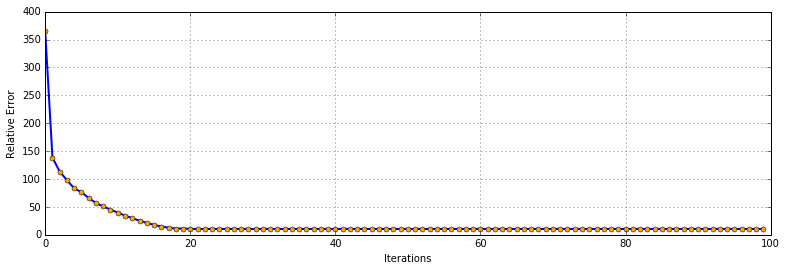
\includegraphics[width=\textwidth]{hpsc_a1_error.png}
    \caption{Error computed with given error function.}
  \end{subfigure}
~
\begin{subfigure}[b]{\textwidth}
    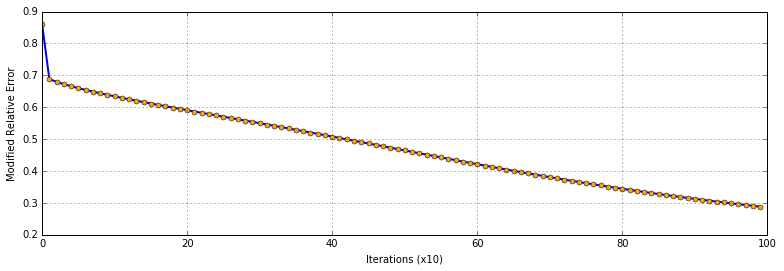
\includegraphics[width=\textwidth]{hpsc_a1_error_rel.png}
    \caption{Error computed with modified error function.}
  \end{subfigure}
  \caption{Convergence of error plot.}
\end{figure*}

As we can see in Figgure 1(a), the error rate is converged to a small value starting from 200 iterations. The difference between 200 iterations and 990 iterations is unclear. On the other hand, in Figure 1(b) - the modified error function, we can see the same type of decrease from 0 to 200 iterations. However, the error rate of this scheme is bounded by 1, and we can clearly see the convergence of higher iterations. Figure 2 demonstrates the result boundary points at 0 interation and 200 iterations. Figure 3 demonstrates boundary points at 990 iterations and 2000 iterations.

\pagebreak

\begin{figure*}[h!]
  \centering
  \begin{subfigure}[b]{0.48\textwidth}
    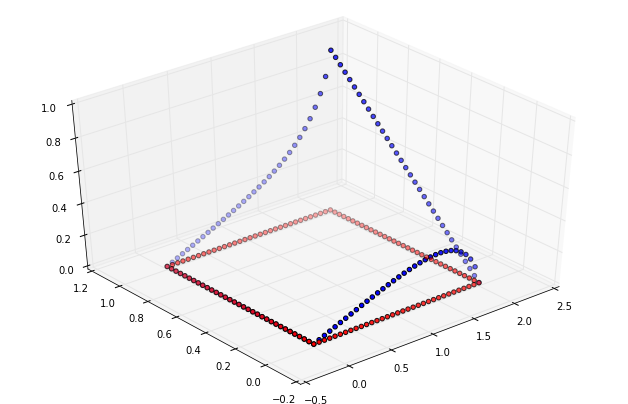
\includegraphics[width=\textwidth]{hpsc_a1_scat_0.png}
    \caption{At 0 iteration. e=364.64, er=0.86.}
  \end{subfigure}
~
\begin{subfigure}[b]{0.48\textwidth}
    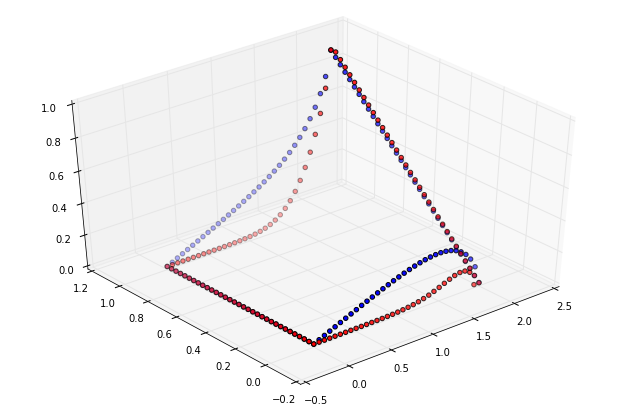
\includegraphics[width=\textwidth]{hpsc_a1_scat_20.png}
    \caption{At 200 iterations. e=10.50, er=0.59.}
  \end{subfigure}
  \caption{Scatter plot of boundary points. e: error; er: error\_rel}
\end{figure*}

\begin{figure*}[h!]
  \centering
  \begin{subfigure}[b]{0.48\textwidth}
    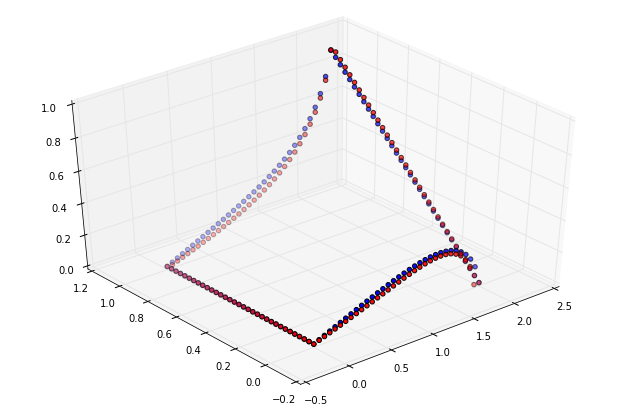
\includegraphics[width=\textwidth]{hpsc_a1_scat_990.png}
    \caption{At 990 iterations. e=10.50, er=0.29}
  \end{subfigure}
~
\begin{subfigure}[b]{0.48\textwidth}
    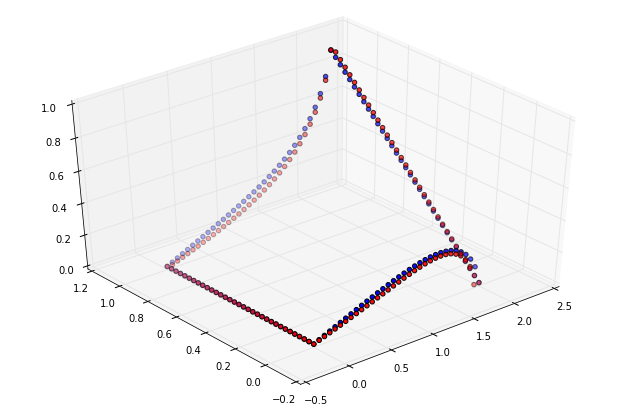
\includegraphics[width=\textwidth]{hpsc_a1_scat_2000.png}
    \caption{At 2000 iterations. e=10.40, er=0.18}
  \end{subfigure}
  \caption{Scatter plot of boundary points. e: error; er: error\_rel}
\end{figure*}
\vfill
\noindent
\emph{The source code and jupyter notebook for this assignment can be found at:} \\
\texttt{https://github.com/gear/HPSC/tree/master/hw}
\end{document}
